% !Mode:: "TeX:UTF-8"
% 七年级上学期第一单元几何体的展开与折叠

\begin{defproblem}{7NJ-04-00-1}%
\begin{onlyproblem}%
如图是一个正方体的表面展开图,如果将它折叠成原来的正方体,那么与点C重合的点是(    )
\begin{center}
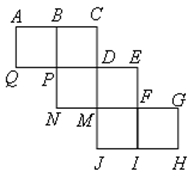
\includegraphics[width=3.5cm]{7NJ01-01-20190804-15}
\end{center}
\xx
{点E和点N}
{点E和点J}
{点H和点A}
{点E和点G}

\end{onlyproblem}%
\begin{onlysolution}%
\begin{solution}%
选D.

解题思路: 要判断点的重合,需先从剪开了一条棱的点处,也就是拐角处进行研究,再从剪开了两条棱的点处判断边如何重合成为棱,最后判断点的重合. 根据正方体一条棱与两个面相连,一条棱被剪开成为两条边,一个顶点连着三条棱,一个顶点属于三个面,在点D所在的拐角处,有两条棱连着,则剩下一条棱被剪开形成两条边DC和DE,因此点E与点C重合. 在点F所在的拐角处,有两条棱连着,则剩下一条棱被剪开形成两条边FE和FG,因此点E与点G重合.所以与点C重合的点为点E和点G,故选D. 
三颗星知识点:正方体的展开与折叠(棱和点)  
\end{solution}%
\end{onlysolution}%
\end{defproblem}


\begin{defproblem}{7NJ-04-00-2}%
\begin{onlyproblem}%
如图是一个正方体的表面展开图,把它折叠成一个正方体时,与点K重合的点是(    ) 
\begin{center}
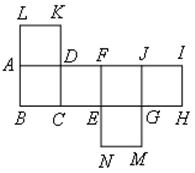
\includegraphics[width=3.5cm]{7NJ01-01-20190804-16}
\end{center}

\xx
{点F}
{点M}
{点F和点N}
{点F和点J}

\end{onlyproblem}%
\begin{onlysolution}%
\begin{solution}%
选A.
解题思路:一个顶点连着三条棱,一个点属于三个面. 如图,
\begin{center}
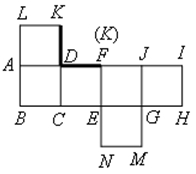
\includegraphics[width=3.5cm]{7NJ01-01-20190804-17}
\end{center}
从拐点D处开始分析,与点D相连的两条棱是连着的,一条棱被剪开,即折叠之后DK与DF重合,那么点K和点F重合,点K属于面ADKL,面CEFD,面EGJF三个面.根据一个点属于三个面,因此与点K重合的点只有点F. 故选A. 
\end{solution}%
\end{onlysolution}%
\end{defproblem}


\begin{defproblem}{7NJ-04-00-3}%
\begin{onlyproblem}%
一个正方体盒子的表面展开图如图所示,如果把它折叠成一个正方体,则点F与点(    )重合. 
\begin{center}
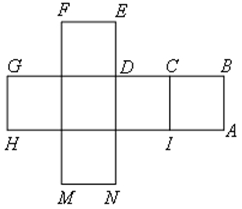
\includegraphics[width=3.5cm]{7NJ01-01-20190804-18}
\end{center}

\xx
{G, H}
{G, M}
{G, B}
{G, D}


\end{onlyproblem}%
\begin{onlysolution}%
\begin{solution}%
选C.
解题思路:要判断点的重合,需先从拐角处进行研究,再从剪开了两条棱的点处研究,判断边和点的重合. 一个顶点连着三条棱,一个点属于三个面. 如图, 
\begin{center}
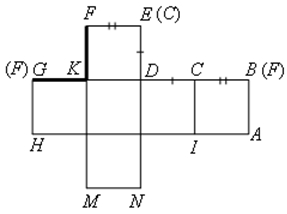
\includegraphics[width=3.5cm]{7NJ01-01-20190804-19}
\end{center}

  左上方的拐点记为K,与点K相连的两条棱是连着的,一条棱被剪开,即折叠之后KG与KF重合,点G和点F重合; 再从拐点D处分析,同样得到点E和点C重合; 接着分析点C,与点C相连的一条棱是连着的,两条棱被剪开,得到四条边CD,CB,ED,EF,已经得出折叠后DE与DC重合,那么剩余的EF与CB重合,所以点F和点B重合.综上,折叠后点F与点G,B重合. 故选C. 
\end{solution}%
\end{onlysolution}%
\end{defproblem}


\begin{defproblem}{7NJ-04-00-4}%
\begin{onlyproblem}%
如图所示的正方体的表面展开图可能是哪一个? 
\begin{center}
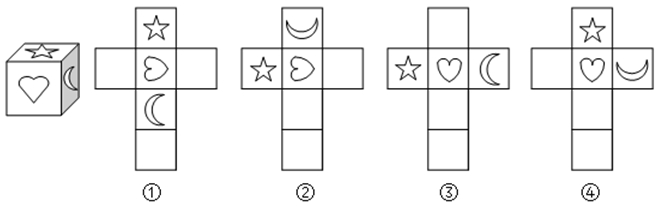
\includegraphics[width=9cm]{7NJ01-01-20190804-20}
\end{center}

\xx
{①}
{②}
{③}
{④}


\end{onlyproblem}%
\begin{onlysolution}%
\begin{solution}%
选②
\end{solution}%
\end{onlysolution}%
\end{defproblem}


\begin{defproblem}{7NJ-04-00-5}%
\begin{onlyproblem}%
如图是一个正方体的表面展开图,则下面四个正方体能由它折叠而成的是哪一个? 
\begin{center}
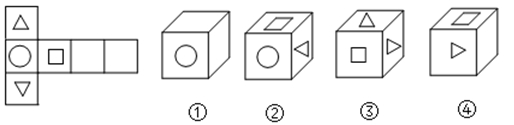
\includegraphics[width=9cm]{7NJ01-01-20190804-21}
\end{center}

\xx
{①}
{②}
{③}
{④}


\end{onlyproblem}%
\begin{onlysolution}%
\begin{solution}%
选④
\end{solution}%
\end{onlysolution}%
\end{defproblem}


\begin{defproblem}{7NJ-04-00-6}%
\begin{onlyproblem}%
如图是一个正方体的表面展开图,这个正方体是(    ) 
\begin{center}
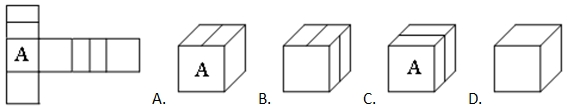
\includegraphics[width=11cm]{7NJ01-01-20190804-22}
\end{center}


\end{onlyproblem}%
\begin{onlysolution}%
\begin{solution}%
选B. 
先从面开始分析,由题可知中间的两个空白面是相对面,根据相对面不可能相邻可知,三个空白面不能同时出现也不能同时不出现,可以排除C,D; 再从棱开始分析,根据展开图可知横线平行于面“A”与横线面相交的棱,排除A,故答案选B. 
\end{solution}%
\end{onlysolution}%
\end{defproblem}



\begin{defproblem}{7NJ-04-00}%
\begin{onlyproblem}%
如图是一个正方体的表面展开图,把它折成正方体后,与边BC重合的边是(    ) 
\begin{center}
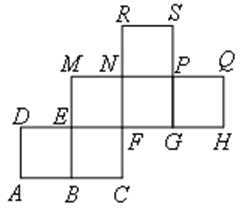
\includegraphics[width=3.5cm]{7NJ01-01-20190804-05}
\end{center}
\xx
{RS}
{HG}
{FG}
{QH}
\end{onlyproblem}%
\begin{onlysolution}%
\begin{solution}%
选B.
要找与边BC重合的边,先找与点B,C重合的点;与面BCFE相对的面是面RSPN,保留这两个面上的点,从拐角处开始分析,通过一条棱与两个面相连,一条棱剪开成为两条边,一个顶点连着三条棱,一个点属于三个面,找到与这些点重合的点,如下图:   则与边BC重合的边为HG,故选B. 
三颗星知识点:正方体的展开与折叠(棱和点)  
\end{solution}%
\end{onlysolution}%
\end{defproblem}



\begin{defproblem}{7NJ-04-01}%
\begin{onlyproblem}%
如图是一个正方体的表面展开图,如果将它折叠成原来的正方体,那么与边LK重合的边是(    ) 
\begin{center}
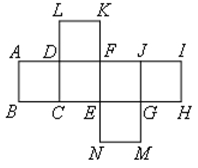
\includegraphics[width=3.5cm]{7NJ01-04-20190803-01.jpg}
\end{center}
\xx
{AB}
{FJ}
{JI}
{MN}
\end{onlyproblem}%
\begin{onlysolution}%
\begin{solution}%
选C.
\begin{center}
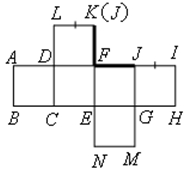
\includegraphics[width=3.5cm]{7NJ01-04-20190803-02.jpg}
\end{center}

要判断边和点的重合,需先从拐角处进行研究,再从剪开了两条棱的点处分析判断边如何重合成为棱. 一条棱与两个面相连,一条棱剪开成为两条边,一个顶点连着三条棱,一个点属于三个面. 如图,   从拐点F处开始分析,与点F相连的两条棱是连着的,剪开了一条棱,即折叠之后FK与FJ重合,点K和点J重合; 接着分析点J,与点J相连的一条棱是连着的,剪开了两条棱,得到四条边JF,JI,KL,KF,已经得出折叠后FK与FJ重合,那么剩余的KL与JI重合,即与边LK重合的边是JI. 故选C. 
\end{solution}%
\end{onlysolution}%
\end{defproblem}





\begin{defproblem}{7NJ-04-02}%
\begin{onlyproblem}%
将下图正方体的相邻两面各划分成九个相同的小正方形,并分别标上“$\circ$”、“$\times$”两符号.若下列有一图形为此正方体的展开图,则此图为(    ) 
\begin{center}
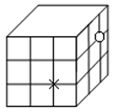
\includegraphics[width=2cm]{7NJ01-04-20190803-03.jpg}
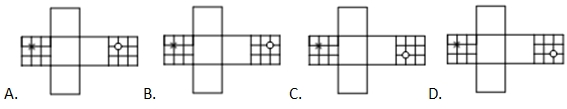
\includegraphics[width=11cm]{7NJ01-04-20190803-10}
\end{center}
\end{onlyproblem}%
\begin{onlysolution}%
\begin{solution}%%
C.
从相对面、相邻面无法判断. 再分析棱,四个展开图经过折叠,带特殊图案的两个面是相邻的.如下图,立体图中面“ABCD”和面“ABEF”有一条重合的棱AB,并且“$\times$”与棱AB的距离是1个网格,“$\circ$”与棱AB的距离是2个网格,可以排除选项B和D; 由于“$\times$”和“$\circ$”距离上下底面的高度不同,排除选项A,故选C. 

\end{solution}%
\end{onlysolution}%
\end{defproblem}



\begin{defproblem}{7NJ-04-03}%
\begin{onlyproblem}%
如图是一个正方体纸盒的表面展开图,下图能由它折叠而成的是哪一个? 
\begin{center}
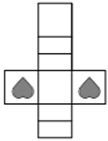
\includegraphics[width=2cm]{7NJ01-04-20190803-11}
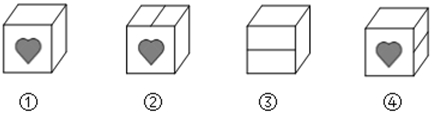
\includegraphics[width=10cm]{7NJ01-04-20190803-05.jpg}
\end{center}
思路分析 

判断正方体展开与折叠问题时,我们按照面、棱、顶点的顺序分析. 首先观察面,由展开图知相对面为“空白对空白”,“横线对横线”,“心对心”;根据“相对面不能相邻”,排除\underline{\hspace*{2cm}}和\underline{\hspace*{2cm}}. 其次研究棱的对应,“心”所在面与“横线”所在面相交于一条棱,根据“心”与这条棱的位置关系可排除\underline{\hspace*{2cm}},应选\underline{\hspace*{2cm}}. 以上横线处依次所填正确的是(    ) 

\xx
{①③④②}
{①④③②}
{①②④③}
{①③②④}
\end{onlyproblem}%
\begin{onlysolution}%
\begin{solution}%%
A.

\end{solution}%
\end{onlysolution}%
\end{defproblem}




\begin{defproblem}{7NJ-04-04}%
\begin{onlyproblem}%
如图所示的正方体的表面展开图可能是(    ) 
\begin{center}
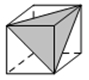
\includegraphics[width=2cm]{7NJ01-04-20190803-06.jpg}
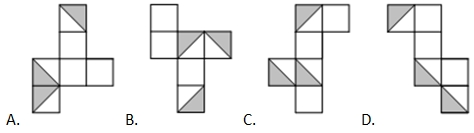
\includegraphics[width=7cm]{7NJ01-04-20190803-07}
\end{center}


\end{onlyproblem}%
\begin{onlysolution}%
\begin{solution}%%
D.
\begin{center}
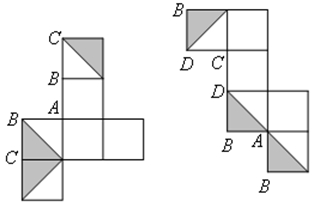
\includegraphics[width=6cm]{7NJ01-04-20190803-08}
\end{center}
先从面开始分析,带阴影的三角形的三个面是相邻面,相邻的面不可能相对,排除选项B和C. 再从棱开始分析,正方体的三个带阴影的直角三角形有公共边,并且有一个公共的顶点是直角顶点,根据一条棱与两个面相连,一条棱被剪开成为两条边,一个顶点连着三条棱,一个顶点属于三个面,分析重合的棱和顶点,选项A和D中重合的边和点如图所示,排除选项A.    故选D. 
\end{solution}%
\end{onlysolution}%
\end{defproblem}



\begin{defproblem}{7NJ-04-05}%
\begin{onlyproblem}%
下列各图都是正方体的表面展开图,若将它们折成正方体,则其中两个正方体各面图案完全一样的是(    ) 
\begin{center}
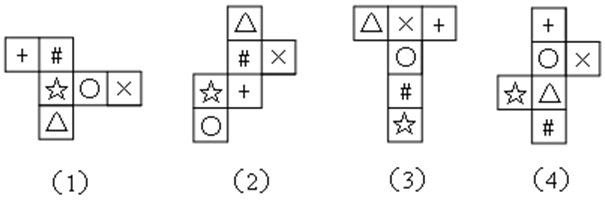
\includegraphics[width=7cm]{7NJ01-01-20190804-04}
\end{center}

\xx
{(1)(2)}
{(2)(3)}
{(3)(4)}
{(2)(4)}

\end{onlyproblem}%
\begin{onlysolution}%
\begin{solution}%%
D.
因为其中有两个正方体折叠之后各面图案完全一样,因此它们对应的平面展开图的相对面必须完全一样.
先分析面“$\triangle$”的相对面:(1)中面“$\triangle$”与面“\#”相对; (2)中面“$\triangle$”与面“$+$”相对; (3)中面“$\triangle$”与面“$+$”相对; (4)中面“$\triangle$”与面“$+$”相对; 因此可排除含有(1)的选项,故排除A;
第二步分析面“$\star$”的相对面: (2)中面“$\star$”与面“$\times$”相对; (3)中面“$\star$”与面“$\circ$”相对; (4)中面“$\star$”与面“$\times$”相对; 因此排除含有(3)的选项,故排除B,C. 经验证(2)和(4)折成的两个正方体各面图案完全一样,故选D.
\end{solution}%
\end{onlysolution}%
\end{defproblem}




\begin{defproblem}{7NJ-04-06}%
\begin{onlyproblem}%
将棱长为1的小正方体组成如图所示的几何体,已知该几何体共由8个小正方体组成,则该几何体的表面积是(    )平方单位. 
\begin{center}
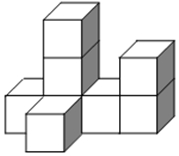
\includegraphics[width=3cm]{7NJ01-04-20190803-09}
\end{center}

\xx
{34}
{32}
{27}
{25}

\end{onlyproblem}%
\begin{onlysolution}%
\begin{solution}%%
A. 根据三视图中小正方体的个数和凹进去的部分, 几何体的表面积为$[(7+4+5) \times 2+2] \times 1^{2}=34$. 故选A. 
\end{solution}%
\end{onlysolution}%
\end{defproblem}





\begin{defproblem}{7NJ-04-07}%
\begin{onlyproblem}%
如图,点M,N,P分别是正方体三条相邻棱的中点,沿着M,N,P三点所在的平面将该正方体的一个角切掉,然后将其展开,其表面展开图可能是(    )  
\begin{center}
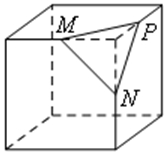
\includegraphics[width=2cm]{7NJ01-01-20190804-06}
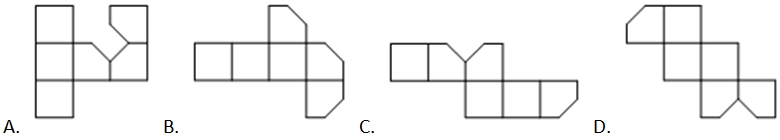
\includegraphics[width=11cm]{7NJ01-01-20190804-07}
\end{center}


\end{onlyproblem}%
\begin{onlysolution}%
\begin{solution}%%
D.
解题思路: 根据正方体的十一种表面展开图可知,没有(3,1,2)型,故排除A; 分析该正方体,缺角的三个面是相邻面,根据相邻面不可能相对排除B; 还可以知道展开之后缺的地方有公共顶点,接着从棱和点开始分析,分析的时候先找出一组相对面标上字母,然后根据边的重合与点的重合标出其他点. C选项中,标出各点的字母如下:   缺的地方没有公共顶点,故C错误; D选项中,标出各点的字母如下:
\begin{center}
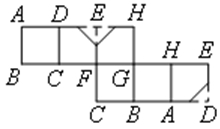
\includegraphics[width=4cm]{7NJ01-01-20190804-08}
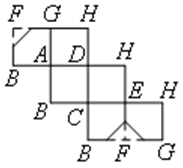
\includegraphics[width=3cm]{7NJ01-01-20190804-09}
\end{center}
 缺的地方有公共顶点,故选D. 
三颗星知识点:正方体的展开与折叠  
\end{solution}%
\end{onlysolution}%
\end{defproblem}




\begin{defproblem}{7NJ-04-08}%
\begin{onlyproblem}%
明明用如图所示的硬纸片折成了一个正方体的盒子,里面装了一瓶墨水,只凭观察,墨水可能在哪个盒子中? 
\begin{center}
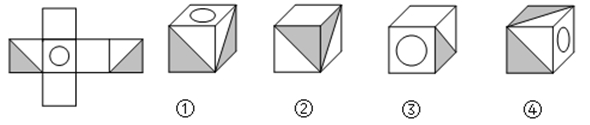
\includegraphics[width=11cm]{7NJ01-01-20190804-10}
\end{center}

思路分析~判断正方体的展开与折叠问题时,我们按照面、棱、顶点的顺序分析. 如图,
\begin{center}
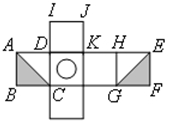
\includegraphics[width=3cm]{7NJ01-01-20190804-11}
\end{center}

首先观察面,展开图中上下两个空白面为相对面,因此这两个空白面不可能同时出现,也不可能同时不出现,因此排除\underline{\hspace*{2cm}}和\underline{\hspace*{2cm}}. 其次研究棱的对应,面ABCD与面“$\circ$”有一条公共棱DC,DC与面ABCD相邻的部分是空白三角形,故排除\underline{\hspace*{2cm}},应选\underline{\hspace*{2cm}}. 以上横线处依次所填正确的是(    ) 

\xx
{①④②③}
{①④③②}
{①③②④}
{①②④③}

\end{onlyproblem}%
\begin{onlysolution}%
\begin{solution}%%
B.
\end{solution}%
\end{onlysolution}%
\end{defproblem}




\begin{defproblem}{7NJ-04-09}%
\begin{onlyproblem}%
如图所示的正方体的表面展开图可能是(    ) 
\begin{center}
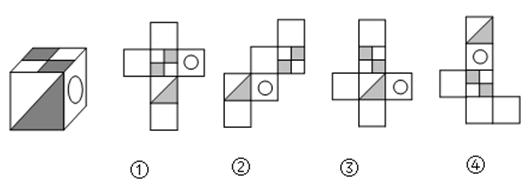
\includegraphics[width=11cm]{7NJ01-01-20190804-12}
\end{center}

思路分析 首先根据“相邻面不可能相对”,排除\underline{\hspace*{2cm}}和\underline{\hspace*{2cm}}. 其次研究棱和顶点的对应,排除\underline{\hspace*{2cm}},应选\underline{\hspace*{2cm}}. 以上横线处依次所填正确的是(    ) 


\xx
{①④②③}
{①④③②}
{②④①③}
{④②③①}

\end{onlyproblem}%
\begin{onlysolution}%
\begin{solution}%%
C.
\end{solution}%
\end{onlysolution}%
\end{defproblem}




\begin{defproblem}{7NJ-04-10}%
\begin{onlyproblem}%
如图是一个正方体的表面展开图,则这个正方体是(    ) 
\begin{center}
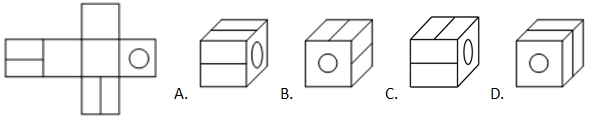
\includegraphics[width=11cm]{7NJ01-01-20190804-13}
\end{center}

\end{onlyproblem}%
\begin{onlysolution}%
\begin{solution}%%
C.
解题思路: 如图,\begin{center}
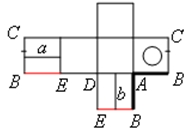
\includegraphics[width=5cm]{7NJ01-01-20190804-14}
\end{center}
先从面开始分析,a,b,“$\circ$”所在的面的为相邻面,从面上无法排除; 然后从棱开始分析,分析的时候从拐角处出发(有两条棱连着的),再分析有一条棱连着的. 由图分析可得在折叠之后的正方体中a所在的面与“$\circ$”所在的面有一条公共棱BC,a与棱BC垂直;b所在的面与“$\circ$”所在的面有一条公共棱AB,b与棱AB平行,故选C. 
\end{solution}%
\end{onlysolution}%
\end{defproblem}






